\documentclass[border=0.2cm]{standalone}
\usepackage{tikz}
\begin{document}


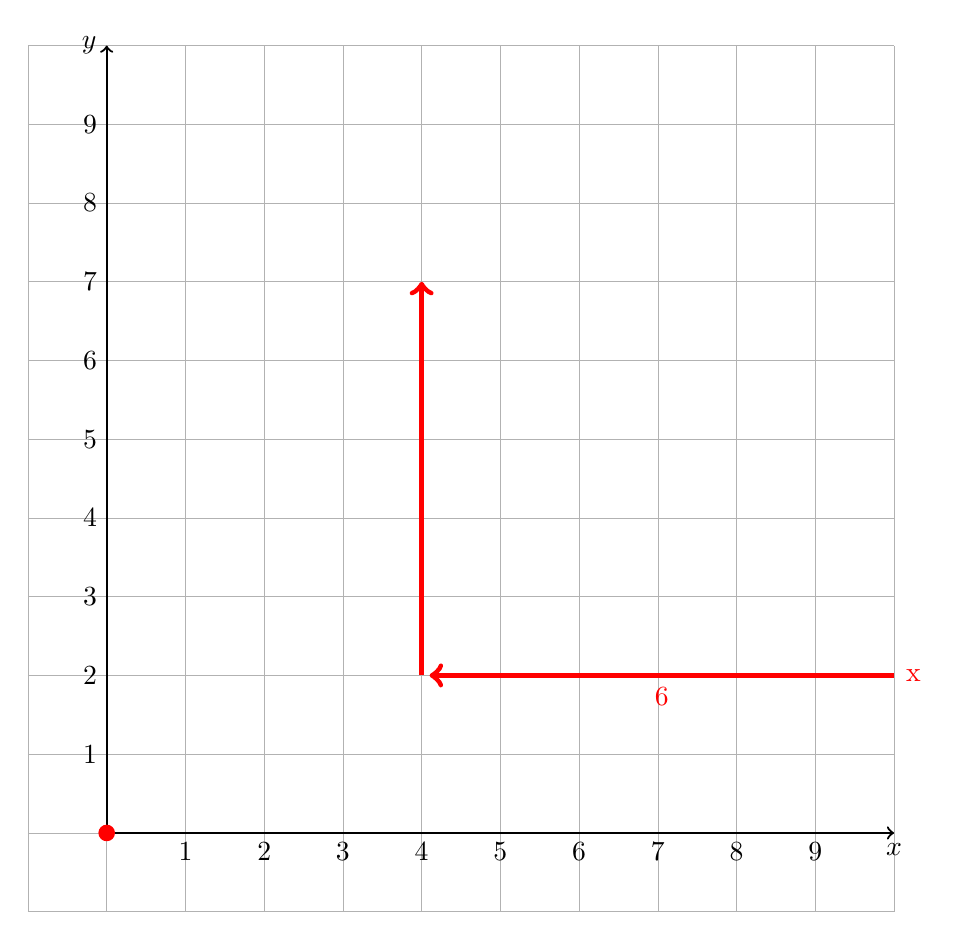
\begin{tikzpicture}
  \draw[help lines,black!30] (-1,-1) grid (10,10);
  \draw[thick,->] (0,0) -- (0,10) node[left]  {$y$};
  \draw[thick,->] (0,0) -- (10,0) node[below] {$x$};
  \foreach \x in {1,...,9} \node[left] at (0,\x) {\x} node[below] at (\x,0) {\x};
  \fill[red] (0,0) circle (3pt); 

  \coordinate (a) at (10,2);
  \coordinate (b) at (6,2);
  \coordinate (c) at (6,7);
  \coordinate (d) at (-3,2);

  
  \draw[line width=2pt,red,->] (10,2) node[right] {x} -- ++(-5.9,0) node[midway,below] {$6$};
  \draw[line width=2pt,red,->] (4,2) -- (4,7);


  %\fill[red] (a) circle (3pt) node[above right] {$Escola$};
  %\fill[red] (b) circle (3pt) node[above right] {$Zoológico$};
  %\fill[red] (c) circle (3pt) node[above right] {$Represa$};
  %\fill[red] (d) circle (3pt) node[above right] {$Igreja$};

  \end{tikzpicture}



\end{document}